\documentclass[a4paper, oneside, 10pt]{article}

\usepackage{amsfonts} % if you want blackboard bold symbols e.g. for real numbers
\usepackage{graphicx} % if you want to include jpeg or pdf pictures

\title{Intelligent RDMA} % change this
\author{Anuj Kalia(akalia)\\
		Yihua Fang(yihuaf)\\
		Xiao Bo Zhao(xiaoboz)}

\date{\today} % change this

\begin{document}

%%%%%%%%%% PRELIMINARY MATERIAL %%%%%%%%%%
\maketitle
\thispagestyle{empty}
\newpage
\begin{center}
\vspace*{\fill}
\section*{Abstract}
The Intelligent RDMA, when presented in plain English, is pretty simple.\\
\vspace*{\fill}
\newpage
\end{center}

%%%%%%%%%% MAIN TEXT STARTS HERE %%%%%%%%%%

\section{Introduction}
Remote Direct Memory Access(RDMA) is a protocol that allows low latency data
sharing across machines connected by a network. Unlike RPC systems, RDMA does
not require control flow transfer by context switches, thereby decreasing both
latency and CPU utilization at the end hosts. Ideally, network adapters
directly link and transfer data between the endpoints' physical memory.
Therefore, there is no copying of data from userspace to kernelspace, further
lowering the latency associated with and data copy.

Since there is no transfer of control flow, the client machine (a host that
reads data from a serevr) must perform all operation on the shared memory
locally. However, operations such as B-tree and linked list traversal, will
require memory access with low locality. As a result, the local machine might
require multiple round-trip times before obtaining its desired data. RPCs do
not suffer from this problem since the server performs this lookup locally and
then transfers the result back to the client. In this scenario, RTTs can easily
dominate the operation cost, nullifying any benefits RDMA gives us.

As a result, we propose an intelligent RDMA that takes into consideration this
indirect memory access use case. Our goal is to minimize the number of RTTs
required to traverse these data structures while maintaining the low context
switching benefits of RDMA. In section 2, we discuss our hypothesis on how to
achieve our goals. In section 3, we present our evaluation methods. In section
4, we outline our schedule and tentative work division. In section 5, we
present our 75\%, 100\%, and 125\% deliverables by the end of this projects.
Finally, in section 6, we will provide the basic outline of our final paper.

\section{Problem with RDMA}
Currently, RDMA only supports basic operations such as RDMA-read and
RDMA-write.  These two operations are great for reading and writing contigeous
memory locations. However, for most modern data access patterns, these basic
operations RDMA offers are inefficient. For example, each get() request for a
B-tree or hash table required 2 RTT, one for grabbing the poiner and one for
reading or writing the data.
\section{Design}
\subsection{Pointer Dereferencing}

The first new operation we added is pointer dereferencing. Given a address and a
length, instead of reading length bytes of data at the address location, we
treat the data stored at location address as pointer. The new operation would
first grab the pointer from location specified by the address and then
dereference the pointer to read/write length bytes to the location.\\

In fact, in our implementation, we allow users to specify the number of
deferencing of the operation. Given the number of dereferencing greater than 1,
the operation would try to dereferencing until it finds the data or report a
invalid memory access error. Before each dereferencing, we implemented a
machanism to check the validity of the pointer the operation is about to
dereferece. Using this machanism, we can avoid to crash the kernel with NULL
pointer or invalid access to memory error.\\

In the traditional RDMA programming model, each dereferencing requires one
additional RTT of communication between the client and the server, one for
obtainning the pointer and one for dereferencing to obtain the data. By
combining the dereferencing into the operation, we save at least half RTT
compared to the traditional RDMA programming model.

\subsection{Conditional Pointer Deferencing}

%TODO: what is the usefulness of the conditional pointer?

\subsection{Scatter Gather}

Scatter gather is another simple operation that can drastically increase the
performance of RDMA operations. Batch operations has long been used in many
systems to improve the performance of operations. Grouping similar operations
together can save overheads and latency.

In our situation, scatter gather is a great operations to have. Batching all
requests into one packets saves RTT and allows the server to process these
requests with more efficiency due to piplining and parallel execution.

\section{Implementation}

% TODO: adding more details???

Since we cannot change the HCA to add new operations for the hardware based
RDMA, we decided to use SoftiWarp, a software based implementation of the RDMA
to prototyping our ideas and proposed solutions.

SoftiWarp reads and writes are handled by the kernel in the form of kernel
module. In the baseline implementation, the kernel module will interprets the
operation, maps the user memory regions into kernel memory, and carefully
performs dereferences.

The SoftiWarp is build on top of TCP and therefore suffer the full latecy of the
data-link layer around 60 $\mu$s. Due to this, the SoftiWarp runs extremely slow
comapred to the hardware based RDMA. However, the SoftiWarp is fully
competitible with the hardware RDMA, which makes it a great prototyping tools
for us to test our theories.

Our implementation modified current read operations to accomidate the pointer
dereferencing by using an used field (uint64\_t wr\_id) to carry required
additional information.

\section{Performance}
In this section, we measured the performance of \emph{SoftiWarp} with newly
added operations. In this section, we will use the following naming conventions
to refer to different implementations we tested.\\
RDMA baseline: The original \emph{SoftiWarp} without any new operations. This
version is used as a baseline to compare to our implementation with additional
operations.\\
RDMA dereferencing: Our implementations of \emph{SoftiWarp} with newly added
operations in dereferencing and conditional dereferencing.\\
RPC: We also implemented a naive RPC packages of cuckoo hashing to be used as a
baseline of comparasion.\\
\subsection{Machine Configuration}
Each machine we used in our testing has 2 AMD Opteron 2.1 GHz processors with 2
GB memory and 1 Gbit Ethernet connections. The operting system on the testing
machine is Ubuntu 12.10. The baseline TCP latency is around 70 $\mu$s.
% TODO: Do we have anything for the link list?? I dont have any data on this....
%\subsection{Link List}

\subsection{Cuckoo Hashing}
We tested our implementation on a cuckoo hash table with 4 million entries. Each
key has equal opportunity to be in either bucket.\\

In the beginning, the client will fill each entries in the hash table. We
measured the performance of each implementation by issuing $2^{20}$ get()
requests of different keys. Then, each attribute is measured and graphed in
figures below.

Below is the graph of average latency of an individual get() request in each
implementation. Note, the latency of the RDMA dereferencing implementation is
approximatly half of the RDMA baseline implementations. This result is exactly
what we perdicted earlier. For each of the get() request, the RDMA baseline
implementation needed to issue 2 requests with 2 RTT, one for the pointer of the
entry and one for obtaining the data inside the entry, whereas the RDMA
dereferencing only require one request with 1 RTT. Effectivly, we improved the
latency of the get() request by a half with the newly add operations.\\

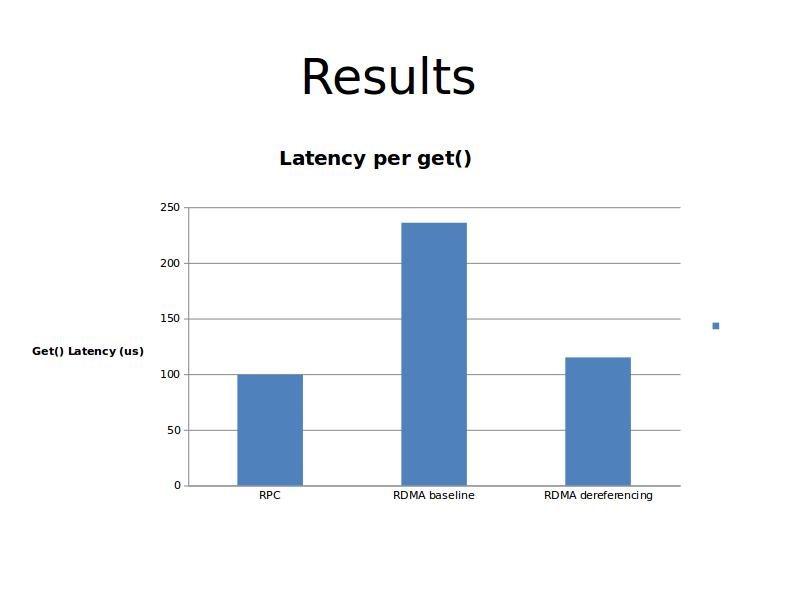
\includegraphics[width=10cm,height=10cm,keepaspectratio]{latency.jpg}

Below is the graph of performance measured in terms of get() requests per
second. Again, we see that there is an 2x improvment from the RDMA baseline to
the RDMA dereferencing. We tested the performance twice, one running 20 client
threads and one running single client thread. The reason we choose to run the
performance test by running 20 client threads is that at 20 threads, the machine
bandwith and CPU usage is just saturated. The number 20 is obtained by running
the test with different number of threads and concluded that 20 is the closest
to fully utilize the machine at hand.

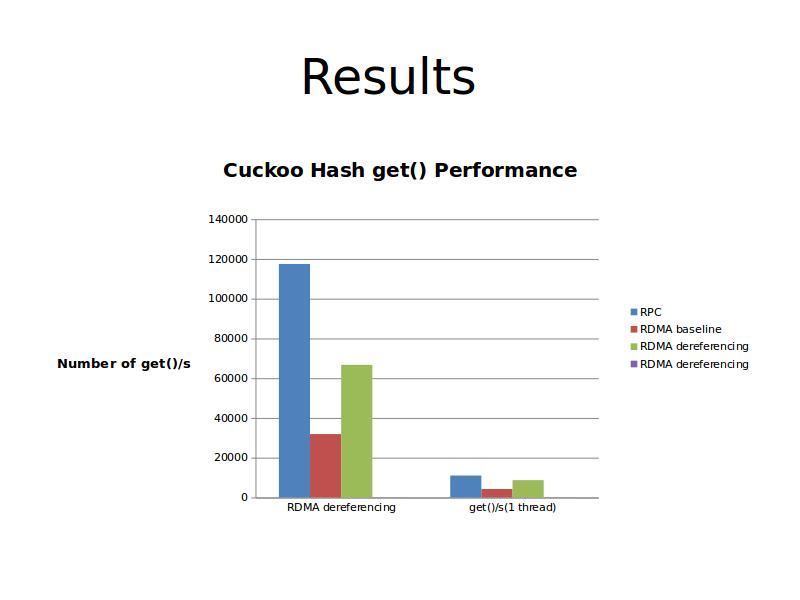
\includegraphics[width=10cm,height=10cm,keepaspectratio]{performance.jpg}
\subsection{Server Kernel Dereferencing Time}

% TODO: we should add in a discussion about RPC because the number shows that RPC is
% far better than softiwarp.
% My understanding is that we only want to use softiwarp for prototyping
% purposes, to test our theory about RDMA in general. We were successful in this
% aspect. However, softiwarp itself is not really practically useful. Our RPC
% implementation can easily beats it. May be we should write about this some
% where?
RPC:\\

Note, although the newly added operations helps to save RTTs in the request, the
server is required to do more work compared to the traditional programming model
of RDMA. Then, naturally, the next question is how much penalty did not server
suffer by adding new operations. In order to investigate this problem, we
measured the server's kernel time spent in dereferencing with different number
of dereferencing per request.\\
% Add figure
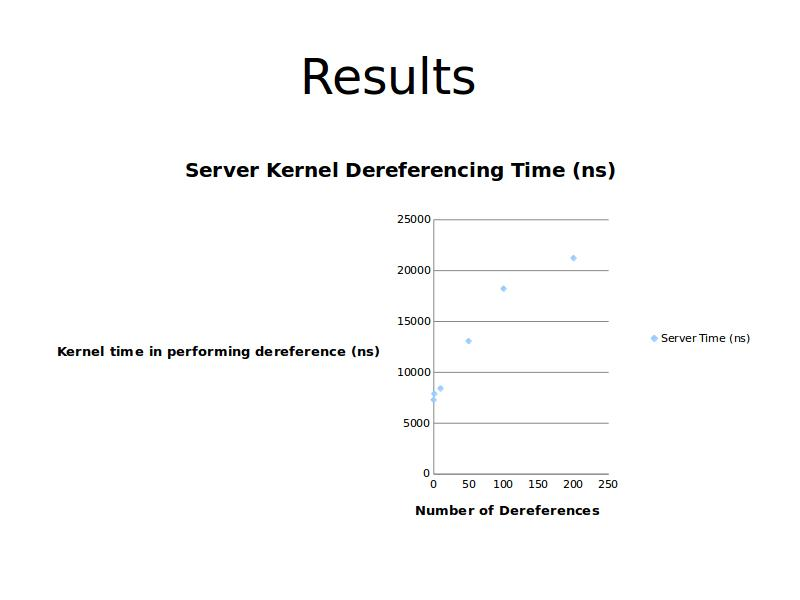
\includegraphics[width=10cm,height=10cm,keepaspectratio]{server_kernel_time.jpg}

\section{Conclusion}

%%%%%%%%%% BIBLIOGRAPHY %%%%%%%%%%
\newpage
\section*{Reference}
%
\begin{description}
% place holder... latex complains when no item...
\item Author, I. (Year). \emph{Book Title}, Publisher; Place of publication.

\end{description}


\bibliographystyle{plain}
\bibliography{references}

\end{document}
